\PassOptionsToPackage{unicode=true}{hyperref} % options for packages loaded elsewhere
\PassOptionsToPackage{hyphens}{url}
\PassOptionsToPackage{dvipsnames,svgnames*,x11names*}{xcolor}
%
\documentclass[11pt]{book}
\usepackage{lmodern}
\usepackage{amssymb,amsmath}
\usepackage{ifxetex,ifluatex}
\usepackage{fixltx2e} % provides \textsubscript
\ifnum 0\ifxetex 1\fi\ifluatex 1\fi=0 % if pdftex
  \usepackage[T1]{fontenc}
  \usepackage[utf8]{inputenc}
  \usepackage{textcomp} % provides euro and other symbols
\else % if luatex or xelatex
  \usepackage{unicode-math}
  \defaultfontfeatures{Ligatures=TeX,Scale=MatchLowercase}
\fi
% use upquote if available, for straight quotes in verbatim environments
\IfFileExists{upquote.sty}{\usepackage{upquote}}{}
% use microtype if available
\IfFileExists{microtype.sty}{%
\usepackage[]{microtype}
\UseMicrotypeSet[protrusion]{basicmath} % disable protrusion for tt fonts
}{}
\IfFileExists{parskip.sty}{%
\usepackage{parskip}
}{% else
\setlength{\parindent}{0pt}
\setlength{\parskip}{6pt plus 2pt minus 1pt}
}
\usepackage{xcolor}
\usepackage{hyperref}
\hypersetup{
            pdftitle={Tidy Modeling with R},
            pdfauthor={Max Kuhn and Davis Vaughan},
            colorlinks=true,
            linkcolor=Maroon,
            filecolor=Maroon,
            citecolor=Blue,
            urlcolor=Blue,
            breaklinks=true}
\urlstyle{same}  % don't use monospace font for urls
\usepackage{color}
\usepackage{fancyvrb}
\newcommand{\VerbBar}{|}
\newcommand{\VERB}{\Verb[commandchars=\\\{\}]}
\DefineVerbatimEnvironment{Highlighting}{Verbatim}{commandchars=\\\{\}}
% Add ',fontsize=\small' for more characters per line
\usepackage{framed}
\definecolor{shadecolor}{RGB}{248,248,248}
\newenvironment{Shaded}{\begin{snugshade}}{\end{snugshade}}
\newcommand{\AlertTok}[1]{\textcolor[rgb]{0.94,0.16,0.16}{#1}}
\newcommand{\AnnotationTok}[1]{\textcolor[rgb]{0.56,0.35,0.01}{\textbf{\textit{#1}}}}
\newcommand{\AttributeTok}[1]{\textcolor[rgb]{0.77,0.63,0.00}{#1}}
\newcommand{\BaseNTok}[1]{\textcolor[rgb]{0.00,0.00,0.81}{#1}}
\newcommand{\BuiltInTok}[1]{#1}
\newcommand{\CharTok}[1]{\textcolor[rgb]{0.31,0.60,0.02}{#1}}
\newcommand{\CommentTok}[1]{\textcolor[rgb]{0.56,0.35,0.01}{\textit{#1}}}
\newcommand{\CommentVarTok}[1]{\textcolor[rgb]{0.56,0.35,0.01}{\textbf{\textit{#1}}}}
\newcommand{\ConstantTok}[1]{\textcolor[rgb]{0.00,0.00,0.00}{#1}}
\newcommand{\ControlFlowTok}[1]{\textcolor[rgb]{0.13,0.29,0.53}{\textbf{#1}}}
\newcommand{\DataTypeTok}[1]{\textcolor[rgb]{0.13,0.29,0.53}{#1}}
\newcommand{\DecValTok}[1]{\textcolor[rgb]{0.00,0.00,0.81}{#1}}
\newcommand{\DocumentationTok}[1]{\textcolor[rgb]{0.56,0.35,0.01}{\textbf{\textit{#1}}}}
\newcommand{\ErrorTok}[1]{\textcolor[rgb]{0.64,0.00,0.00}{\textbf{#1}}}
\newcommand{\ExtensionTok}[1]{#1}
\newcommand{\FloatTok}[1]{\textcolor[rgb]{0.00,0.00,0.81}{#1}}
\newcommand{\FunctionTok}[1]{\textcolor[rgb]{0.00,0.00,0.00}{#1}}
\newcommand{\ImportTok}[1]{#1}
\newcommand{\InformationTok}[1]{\textcolor[rgb]{0.56,0.35,0.01}{\textbf{\textit{#1}}}}
\newcommand{\KeywordTok}[1]{\textcolor[rgb]{0.13,0.29,0.53}{\textbf{#1}}}
\newcommand{\NormalTok}[1]{#1}
\newcommand{\OperatorTok}[1]{\textcolor[rgb]{0.81,0.36,0.00}{\textbf{#1}}}
\newcommand{\OtherTok}[1]{\textcolor[rgb]{0.56,0.35,0.01}{#1}}
\newcommand{\PreprocessorTok}[1]{\textcolor[rgb]{0.56,0.35,0.01}{\textit{#1}}}
\newcommand{\RegionMarkerTok}[1]{#1}
\newcommand{\SpecialCharTok}[1]{\textcolor[rgb]{0.00,0.00,0.00}{#1}}
\newcommand{\SpecialStringTok}[1]{\textcolor[rgb]{0.31,0.60,0.02}{#1}}
\newcommand{\StringTok}[1]{\textcolor[rgb]{0.31,0.60,0.02}{#1}}
\newcommand{\VariableTok}[1]{\textcolor[rgb]{0.00,0.00,0.00}{#1}}
\newcommand{\VerbatimStringTok}[1]{\textcolor[rgb]{0.31,0.60,0.02}{#1}}
\newcommand{\WarningTok}[1]{\textcolor[rgb]{0.56,0.35,0.01}{\textbf{\textit{#1}}}}
\usepackage{longtable,booktabs}
% Fix footnotes in tables (requires footnote package)
\IfFileExists{footnote.sty}{\usepackage{footnote}\makesavenoteenv{longtable}}{}
\usepackage{graphicx,grffile}
\makeatletter
\def\maxwidth{\ifdim\Gin@nat@width>\linewidth\linewidth\else\Gin@nat@width\fi}
\def\maxheight{\ifdim\Gin@nat@height>\textheight\textheight\else\Gin@nat@height\fi}
\makeatother
% Scale images if necessary, so that they will not overflow the page
% margins by default, and it is still possible to overwrite the defaults
% using explicit options in \includegraphics[width, height, ...]{}
\setkeys{Gin}{width=\maxwidth,height=\maxheight,keepaspectratio}
\setlength{\emergencystretch}{3em}  % prevent overfull lines
\providecommand{\tightlist}{%
  \setlength{\itemsep}{0pt}\setlength{\parskip}{0pt}}
\setcounter{secnumdepth}{5}
% Redefines (sub)paragraphs to behave more like sections
\ifx\paragraph\undefined\else
\let\oldparagraph\paragraph
\renewcommand{\paragraph}[1]{\oldparagraph{#1}\mbox{}}
\fi
\ifx\subparagraph\undefined\else
\let\oldsubparagraph\subparagraph
\renewcommand{\subparagraph}[1]{\oldsubparagraph{#1}\mbox{}}
\fi

% set default figure placement to htbp
\makeatletter
\def\fps@figure{htbp}
\makeatother

\usepackage{etoolbox}
\makeatletter
\providecommand{\subtitle}[1]{% add subtitle to \maketitle
  \apptocmd{\@title}{\par {\large #1 \par}}{}{}
}
\makeatother
% Begin preamble.tex -----------------------------------------------------------

% ------------------------------------------------------------------------------
% size based on "Statistical Rethinking" style files

\usepackage[paperwidth=7.67in,paperheight=10.67in,layoutwidth=7in,layoutheight=10in,text={5.5in,8.5in},left=0.65in,top=0.75in,headheight=0.25in,headsep=0.4in,footskip=0.4in,showcrop, layouthoffset=0.33in, layoutvoffset=0.33in]{geometry}

% ------------------------------------------------------------------------------
% headers

\usepackage{fancyhdr}

\pagestyle{fancy}
\fancyhf{}
\fancyhead[CO]{\nouppercase{\emph{\rightmark}}}
\fancyhead[CE]{\nouppercase{\emph{\leftmark}}}
\fancyhead[RO]{\thepage}
\fancyhead[LE]{\thepage}
% no line in header or footer
\renewcommand{\headrulewidth}{0pt}

% Code chunk mods -------------------------------------------------------------
\DefineVerbatimEnvironment{Highlighting}{Verbatim}{commandchars=\\\{\},fontsize=\small}
\renewcommand{\CommentTok}[1]{\textcolor[rgb]{0.41,0.41,0.41}{\texttt{#1}}}



% End preamble.tex -------------------------------------------------------------
% https://github.com/rstudio/rmarkdown/issues/337
\let\rmarkdownfootnote\footnote%
\def\footnote{\protect\rmarkdownfootnote}

% https://github.com/rstudio/rmarkdown/pull/252
\usepackage{titling}
\setlength{\droptitle}{-2em}

\pretitle{\vspace{\droptitle}\centering\huge}
\posttitle{\par}

\preauthor{\centering\large\emph}
\postauthor{\par}

\predate{\centering\large\emph}
\postdate{\par}
\usepackage[]{natbib}
\bibliographystyle{apalike}

\title{Tidy Modeling with R}
\author{Max Kuhn and Davis Vaughan}
\date{2020-01-09}

\begin{document}
\maketitle

{
\hypersetup{linkcolor=}
\setcounter{tocdepth}{1}
\tableofcontents
}
\hypertarget{hello-world}{%
\chapter*{Hello World}\label{hello-world}}
\addcontentsline{toc}{chapter}{Hello World}

This is the website for \emph{Tidy Modeling with R}. Its purpose is to be a guide to using a new collection of software in the R programming language that enable model building. There are few goals, depending on your background. First, if you are new to modeling and R, we hope to provide an introduction on how to use our software to create models. The focus will be on a dialect of R called \emph{the tidyverse} that is designed to be a better interface for common tasks using R. If you've never heard of the tidyverse, there is a chapter that provides a solid introduction. The second (and primary) goal is to demonstrate how the tidyverse can be used to produce high quality models. The tools used to do this are referred to as the \emph{tidymodels packages}. The third goal is to use the tidymodels packages to encourage good methodology and statistical practice. Many models, especially complex predictive or machine learning models, can work very well on the data at hand but may also fail when exposed to new data. Often, this issue is due to poor choices that were made during the development and/or selection of the models. Whenever possible, our software attempts to prevent these and other pitfalls.

This book is not intended to be a reference on different types of these techniques We suggest other resources to learn the nuances of models. A general source for information about the most common type of model, the \emph{linear model}, we suggest \citet{fox08}. Another excellent resource for investigating and analyzing data is \citet{wickham2016}. For predictive models, \citet{apm} is a good resource. For pure machine learning methods, \citet{Goodfellow} is an excellent (but formal) source of information. In some cases, we describe some models that are used in this text but in a way that is less mathematical (and hopefully more intuitive).

We do not assume that readers will have had extensive experience in model building and statistics. Some statistical knowledge is required, such as: random sampling, variance, correlation, basic linear regression, and other topics that are usually found in a basic undergraduate statistics or data analysis course.

\emph{Tidy Modeling with R} is currently a work in progress. As we create it, this website is updated. Be aware that, until it is finalized, the content and/or structure of the book may change.

This openness also allows users to contribute if they wish. Most often, this comes in the form of correcting typos, grammar, and other aspects of our work that could use improvement. Instructions for making contributions can be found in the \href{https://github.com/topepo/TMwR/blob/master/contributing.md}{\texttt{contributing.md}} file. Also, be aware that this effort has a code of conduct, which can be found at \href{https://github.com/topepo/TMwR/blob/master/code_of_conduct.md}{\texttt{code\_of\_conduct.md}}.

In terms of software lifecycle, the tidymodels packages are fairly young. We will do our best to maintain backwards compatibility and, at the completion of this work, will archive the specific versions of software that were used to produce it. The primary packages, and their versions, used to create this website are:

\begin{verbatim}
#> - Session info ---------------------------------------------------------------
#>  setting  value                       
#>  version  R version 3.6.1 (2019-07-05)
#>  os       macOS Catalina 10.15.1      
#>  system   x86_64, darwin15.6.0        
#>  ui       X11                         
#>  language (EN)                        
#>  collate  en_US.UTF-8                 
#>  ctype    en_US.UTF-8                 
#>  tz       America/New_York            
#>  date     2020-01-09                  
#> 
#> - Packages -------------------------------------------------------------------
#>  package     * version    date       lib source                      
#>  AmesHousing * 0.0.3      2017-12-17 [1] CRAN (R 3.6.0)              
#>  bookdown    * 0.16       2019-11-22 [1] CRAN (R 3.6.0)              
#>  broom         0.5.3      2019-12-14 [1] CRAN (R 3.6.0)              
#>  dplyr       * 0.8.3      2019-07-04 [1] CRAN (R 3.6.0)              
#>  ggplot2     * 3.2.1      2019-08-10 [1] CRAN (R 3.6.0)              
#>  purrr       * 0.3.3      2019-10-18 [1] CRAN (R 3.6.0)              
#>  rlang         0.4.2.9000 2019-12-26 [1] Github (r-lib/rlang@ce4f717)
#>  tibble      * 2.1.3      2019-06-06 [1] CRAN (R 3.6.0)              
#> 
#> [1] /Library/Frameworks/R.framework/Versions/3.6/Resources/library
\end{verbatim}

\href{https://pandoc.org/}{\texttt{pandoc}} is also instrumental in creating this work. The version used here is 2.3.1.

\hypertarget{introduction}{%
\chapter{Introduction}\label{introduction}}

Models are mathematical tools that create equations that are intended to mimic the data given to them. These equations can be used for various purposes, such as: predicting future events, determining if there is a difference between several groups, as an aid to a map-based visualization, discovering novel patterns in the data that could be further investigated, and so on. Their utility hinges on their ability to be reductive; the primary influences in the data can be captured mathematically in a way that is useful.

Since the start of the 21st century, mathematical models have become ubiquitous in our daily lives, in both obvious and subtle ways. A typical day for many people might involve checking the weather to see when a good time would be to walk the dog, ordering a product from a website, typing (and autocorrecting) a text message to a friend, and checking email. In each of these instances, there is a good chance that some type of model was used in an assistive way. In some cases, the contribution of the model might be easily perceived (``You might also be interested in purchasing product \emph{X}'') while in other cases the impact was the absence of something (e.g., spam email). Models are used to choose clothing that a customer might like, a molecule that should be evaluated as a drug candidate, and might even be the mechanism that a nefarious company uses avoid the discovery of cars that over-pollute. For better or worse, models are here to stay.

Two reasons that models permeate our lives are that software exists that facilitates their creation and that data has become more easily captured and accessible. In regard to software, it is obviously critical that software produces the \emph{correct} equations that represent the data. For the most part, determining mathematical correctness is possible. However, the creation of an appropriate model hinges on a few other aspects.

First, it is important that it is easy to operate the software in a \emph{proper way}. For example, the user interface should not be so arcane that the user would not know that they have inappropriately specified the wrong information. As an analogy, one might have a high quality kitchen measuring cup capable of great precision but if the chef adds a cup of salt instead of a cup of sugar, the results would be unpalatable. As a specific example of this issue, \citet{baggerly2009} report myriad problems in the data analysis in a high profile computational biology publication. One of the issues was related to how the users were required to add the names of the model inputs. The user-interface of the software was poor enough that it was easy to \emph{offset} the column names of the data from the actual data columns. In the analysis of the data, this resulted in the wrong genes being identified as important for treating cancer patients. This, and many other issues, led to the stoppage of numerous clinical trials \citep{Carlson2012}.

If we are to expect high quality models, it is important that the software facilitate proper usage. \citet{abrams2003} describes an interesting principle to live by:

\begin{quote}
The Pit of Success: in stark contrast to a summit, a peak, or a journey across a desert to find victory through many trials and surprises, we want our customers to simply fall into winning practices by using our platform and frameworks.
\end{quote}

Data analysis software should also espouse this idea.

The second important aspect of model building is related to \emph{scientific methodology}. For models that are used to make complex predictions, it can be easy to unknowingly commit errors related to logical fallacies or inappropriate assumptions. Many machine learning models are so adept at finding patterns, they can effortlessly find empirical patterns in the data that fail to reproduce later. Some of these types of methodological errors are insidious in that the issue might be undetectable until a later time when new data that contain the true result are obtained. In short, as our models become more powerful and complex it has also become easier to commit latent errors. This also relates to programming. Whenever possible, the software should be able to protect users from committing such mistakes. Software should make it easy for users to do the right thing.

These two aspects of model creation are crucial. Since tools for creating models are easily obtained and models can have such a profound impact, many more people are creating them. In terms of technical expertise and training, their backgrounds will vary. It is important that their tools be \emph{robust} to the experience of the user. On one had, they tools should be powerful enough to create high-performance models but, on the other hand, should be easy to use in an appropriate way. This book describes a suite of software that can can create different types of models. The software has been designed with these additional characteristics in mind.

The software is based on the R programming language \citep{baseR}. R has been designed especially for data analysis and modeling. It is based on the \emph{S language} which was created in the 1970's to

\begin{quote}
``turn ideas into software, quickly and faithfully'' \citep{Chambers:1998}
\end{quote}

R is open-source and is provided free of charge. It is a powerful programming language that can be used for many different purposes but specializes in data analysis, modeling, and machine learning. R is easily \emph{extensible}; it has a vast ecosystem of \emph{packages}; these are mostly user-contributed modules that focus on a specific theme, such as modeling, visualization, and so on.

One collection of packages is called the \textbf{\emph{tidyverse}} \citep{tidyverse}. The tidyverse is an opinionated collection of R packages designed for data science. All packages share an underlying design philosophy, grammar, and data structures. Several of these design philosophies are directly related to the aspects of software described above. If you've never used the tidy verse packages, Chapter \ref{tidyverse-primer} contains a review. Within the tidyverse, there is a set of packages specifically focused on modeling and these are usually referred to as the \textbf{\emph{tidymodels}} packages. This book is an extended software manual for conducting modeling using the tidyverse. It shows how to use a set of packages, each with its own specific purpose, together to create high-quality models.

\hypertarget{types-of-models}{%
\section{Types of models}\label{types-of-models}}

Before proceeding, lets describe a taxa for types of models, grouped by \emph{purpose}. While not exhaustive, most models fail into \emph{at least} one of these categories:

\textbf{Descriptive Models}: The purpose here would be to model the data so that it can be used to describe or illustrate characteristics of some data. The analysis might have no other purpose than to visually emphasize some trend or artifact in the data.

For example, large scale measurements of RNA have been possible for some time using \emph{microarrays}. Early laboratory methods placed a biological sample on a small microchip. Very small locations on the chip would be able to assess a measure of signal based on the abundance of a specific RNA sequence. The chip would contain thousands (or more) outcomes, each a quantification of the RNA related to some biological process. However, there could be quality issued on the chip that might lead to poor results. A fingerprint accidentally left on a portion of the chip might cause inaccurate measurements when scanned.

An early methods for evaluating such issues where \emph{probe-level models}, or PLM's \citep{bolstad2004}. A statistical model would be created that accounted for the \emph{known} differences for the data from the chip, such as the RNA sequence, the type of sequence and so on. If there were other, unwanted factors in the data, these would be contained in the model residuals. When the residuals were plotted by their location on the chip, a good quality chip would show no patterns. When an issue did occur, some sort of spatial pattern would be discernible. Often the type of pattern would suggest the underlying issue (e.g.~a fingerprint) and a possible solution (wipe the chip off and rescan). Figure \ref{fig:descr-examples}(a) shows an application of this method for two microarrays taken from \citet{Gentleman2005}. The images show two different colors; red is where the signal intensity was larger than the model expects while the blue color shows lower than expected values. The left-hand panel demonstrates a fairly random pattern while the right-hand panel shows some type of unwanted artifact.

\begin{figure}

{\centering \includegraphics[width=0.8\linewidth]{figures/introduction-descr-examples-1} 

}

\caption{Two examples of how descriptive models can be used to illustrate specific patterns.}\label{fig:descr-examples}
\end{figure}

Another example of a descriptive model is the \emph{locally estimated scatterplot smoothing} model, more commonly known as LOESS \citep{cleveland1979}. Here, a smooth and flexible regression model is fit to a data set, usually with a single independent variable, and the fitted regression line is used to elucidate some trend in the data. These types of \emph{smoothers} are used to discover potential ways to represent a variable in a model. This is demonstrated in Figure \ref{fig:descr-examples}(b) where a nonlinear trend is illuminated by the flexible smoother.

\textbf{Inferential Models}: In these situations, the goal is to produce a decision for a research question or to test a specific hypothesis. The goal is to make some statement of truth regarding some predefined conjecture or idea. In many (but not all) cases, some qualitative statement is produced.

For example, in a clinical trial, the goal might be to provide confirmation that a new therapy does a better job in prolonging life than an alternative (e.g., an existing therapy or no treatment). If the clinical endpoint was related to survival or a patient, the \emph{null hypothesis} might be that the two therapeutic groups have equal median survival times with the alternative hypothesis being that the new therapy has higher median survival. If this trial were evaluated using the traditional \emph{null hypothesis significance testing} (NHST), a p-value would be produced using some pre-defined methodology based on a set of assumptions for the data. Small values of the p-value indicate that there is evidence that the new therapy does help patients live longer. If not, the conclusion is that there is a failure to show such an difference (which could be due to a number of reasons).

What are the important aspects of this type of analysis? Inferential techniques typically produce some type of probabilistic output, such as a p-value, confidence interval, or posterior probability. Generally, to compute such a quantity, formal assumptions must be made about the data and the underlying processes that generated the data. The quality of the statistical results are highly dependent on these pre-defined assumptions as well as how much the observed data appear to agree with them. The most critical factors here are theoretical in nature: if my data were independent and follow distribution \emph{X}, then test statistic \emph{Y} can be used to produce a p-value. Otherwise, the resulting p-value might be inaccurate.

One aspect of inferential analyses is that there \emph{tends} to be a longer feedback loop that could help understand how well the data fit the assumptions. In our clinical trial example, if statistical (and clinical) significance indicated that the new therapy should be available for patients to use, it may be years before it is used in the field and enough data were generated to have an independent assessment of whether the original statistical analysis led to the appropriate decision.

\textbf{Predictive Models}: There are occasions where data are modeled in an effort to produce the most accurate prediction possible for new data. Here, the primary goal is that the predicted values have the highest possible fidelity to the true value of the new data.

A simple example would be for a book buyer to predict how many copies of a particular book should be shipped to his/her store for the next month. An over-prediction wastes space and money due to excess books. If the prediction is smaller than it should be, there is opportunity loss and less profit.

For this type of model, the problem type is one of \emph{estimation} rather than inference. For example, the buyer is usually not concerned with a question such as ``Will I sell more than 100 copies of book \emph{X} next month?'' but rather ``How many copies of \emph{X} will customers purchase next month?'' Also, depending on the context, there may not be any interest in \emph{why} the predicted value is \emph{X}. In other words, is more interest in the value itself than evaluating a formal hypothesis related to the data. That said, the prediction can also include measures of uncertainty. In the case of the book buyer, some sort of forecasting error might be valuable to help them decide on how many to purchase or could serve as a metric to gauge how well the prediction method worked.

What are the most important factors affecting predictive models? There are many different ways that a predictive model could be created. The important factors depend on how the model was developed.

For example, a \emph{mechanistic model} could be developed based on first principles to produce a model equation that is dependent on assumptions. For example, when predicting the amount of a drug that is in a person's body at a certain time, some formal assumptions are made on how the drug is administered, absorbed, metabolized, and eliminated. Based on this, a set of differential equations can be used to derive a specific model equation. Data are used to estimate the known parameters of this equation and predictions are made after parameter estimation. Like inferential models, mechanistic predictive models greatly depend on the assumptions that define their model equations. However, unlike inferential models, it is easy to make data-driven statements about how well the model performs based on how well it predicts the existing data. Here the feedback loop for the modeler is much faster than it would be for a hypothesis test.

\emph{Empirically driven models} are those that have more vague assumptions that are used to create their model equations. These models tend to fall more into the machine learning category. A good example is the simple \emph{K}-nearest neighbor (KNN) model. Given a set of reference data, a new sample is predicted by using the values of the most similar data in the reference set. For example, if a book buyer needs a prediction for a new book, historical data from existing books may be available. A 5-nearest neighbor model would estimate the amount of the new book to purchase based on the sales numbers of the five books that are most similar to the new one (for some definition of ``similar''). This model is only defined by the structure of the prediction (the average of five similar books). No theoretical or probabilistic assumptions are made about the sales numbers or the variables that are used to define similarity. In fact, the primary method of evaluating the appropriateness of the model is to assess its accuracy using existing data. If the structure of this type of model was a good choice, the predictions would not be close to the actual values.

Broader discussions of these distinctions can be found in \citet{breiman2001} and \citet{shmueli2010}. Note that we have defined the type of model by how it is used rather than its mathematical qualities. An ordinary linear regression model might fall into all three classes of models, depending on how it is used:

\begin{itemize}
\item
  Descriptive smoother, similar to LOESS, called \emph{restricted smoothing splines} \citep{Durrleman1989} can be used to describe trends in data using ordinary linear regression with specialized terms.
\item
  An \emph{analysis of variance} (ANOVA) model is a popular method for producing the p-values used for inference. ANOVA models are a special case of linear regression.
\item
  If a simple linear regression model produces highly accurate predictions, it can be used as a predictive model.
\end{itemize}

However, there are many more examples of predictive models that cannot (or at least should not) be used for inference. Even if probabilistic assumptions were made for the data, the nature of the KNN model makes the math required for inference intractable.

There is an additional connection between the types of models. While the primary purpose of descriptive and inferential models might not be related to prediction, the predictive capacity of the model should not be ignored. For example, logistic regression is a popular model for data where the outcome is qualitative with two possible values. It can model how variables related to the probability of the outcomes. When used in an inferential manner, there is usually an abundance of attention paid to the \emph{statistical qualities} of the model. For example, analysts tend to strongly focus on the selection of which independent variables are contained in the model. Many iterations of model building are usually used to determine a minimal subset of independent variables that have a ``statistically significant'' relationship to the outcome variable. This is usually achieved when all of the p-values for the independent variables are below some value (e.g.~0.05). From here, the analyst typically focuses on making qualitative statements about the relative influence that the variables have on the outcome.

A potential problem with this approach is that it can be dangerous when statistical significance is used as the \emph{only} measure of model quality. It is certainly possible that this statistically optimized model has poor model accuracy (or some other measure of predictive capacity). While the model might not be used for prediction, how much should the inferences be trusted from a model that has all significant p-values but a dismal accuracy? Predictive performance tends to be related to how close the model's fitted values are to the observed data. If the model has limited fidelity to the data, the inferences generated by the model should be highly suspect. In other words, statistical significance may not imply that the model should be used. This may seem intuitively obvious, but is often ignored in real-world data analysis.

\hypertarget{some-terminology}{%
\section{Some terminology}\label{some-terminology}}

Before proceeding, some additional terminology related to modeling, data, and other quantities should be outlined. These descriptions are not exhaustive.

First, many models can be categorized as being \emph{supervised} or \emph{unsupervised}. Unsupervised models are those that seek patterns, clusters, or other characteristics of the data but lack an outcome variable (i.e., a dependent variable). For example, principal component analysis (PCA), clustering, and autoencoders are used to understand relationships between variables or sets of variables without an explicit relationship between variables and an outcome. Supervised models are those that have an outcome variable. Linear regression, neural networks, and numerous other methodologies fall into this category. Within supervised models, the two main sub-categories are:

\begin{itemize}
\item
  \emph{Regression}, where a numerical outcome is being predicted.
\item
  \emph{Classification}, where the outcome is an ordered or unordered set of \emph{qualitative} values.
\end{itemize}

These are imperfect definitions and do not account for all possible types of models. In coming chapters, we refer to these types of supervised techniques as the \emph{model mode}.

In terms of data, the main species are quantitative and qualitative. Examples of the former are real numbers and integers. Qualitative values, also known as nominal data, are those that represent some sort of discrete state that cannot be placed on a numeric scale.

Different variables can have different \emph{roles} in an analysis. Outcomes (otherwise known as the labels, endpoints, or dependent variables) are the value being predicted in supervised models. The independent variables, which are the substrate for making predictions of the outcome, also referred to as predictors, features, or covariates (depending on the context). Here, the terms \emph{outcomes} and \emph{predictors} are used most frequently here.

\hypertarget{model-phases}{%
\section{How does modeling fit into the data analysis/scientific process?}\label{model-phases}}

In what circumstances are model created? Are there steps that precede such an undertaking? Is it the first step in data analysis?

There are always a few critical phases of data analysis that come before modeling. First, there is the chronically underestimated process of \textbf{cleaning the data}. No matter the circumstances, the data should be investigated to make sure that it is well understood, applicable to the project goals, accurate, and appropriate. These steps can easily take more time than the rest of the data analysis process (depending on the circumstances).

Data cleaning can also overlap with the second phase of \textbf{understanding the data}, often referred to as exploratory data analysis (EDA). There should be knowledge of how the different variables related to one another, their distributions, typical ranges, and other attributes. A good question to ask at this phase is ``how did I come by \emph{these} data?'' This question can help understand how the data at-hand have been sampled or filtered and if these operations were appropriate. For example, when merging data base tables, a join may go awry that could accidentally eliminate one or more sub-populations of samples. Another good idea would be to ask if the data are \emph{relavant}. For example, to predict whether patients have Alzheimer's disease or not, it would be unwise to have a data set containing subject with the disease and a random sample of healthy adults from the general population. Given the progressive nature of the disease, the model my simply predict who the are the \emph{oldest patients}.

Finally, before starting a data analysis process, there should be clear expectations of the goal of the model and how performance (and success) will be judged. At least one \emph{performance metric} should be identified with realistic goals of what can be achieved. Common statistical metrics are classification accuracy, true and false positive rates, root mean squared error, and so on. The relative benefits and drawbacks of these metrics should be weighted. It is also important that the metric be germane (i.e., alignment with the broader data analysis goals is critical).

\begin{figure}

{\centering 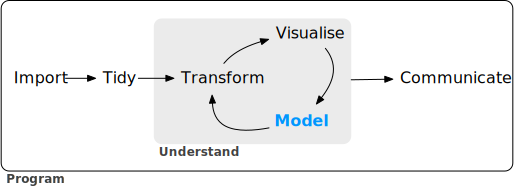
\includegraphics[width=0.8\linewidth]{figures-premade/data-science-model} 

}

\caption{The data science process (from R for Data Science).}\label{fig:data-science-model}
\end{figure}

The process of investigating the data may not be simple. \citet{wickham2016} contains an excellent illustration of the general data analysis process, reproduced with Figure \ref{fig:data-science-model}. Data ingestion and cleaning are shown as the initial steps. When the analytical steps commence, they are a heuristic process; we cannot pre-determine how long they may take. The cycle of analysis, modeling, and visualization often require multiple iterations.

\begin{figure}

{\centering 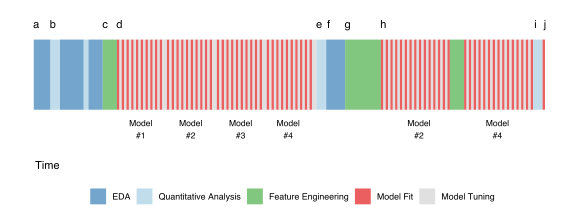
\includegraphics[width=1\linewidth]{figures/introduction-modeling-process-1} 

}

\caption{A schematic for the typical modeling process (from Feature Engineering and Selection).}\label{fig:modeling-process}
\end{figure}

This iterative process is especially true for modeling. Figure \ref{fig:modeling-process} originates from \citet{kuhn20202} and is meant to emulate the typical path to determining an appropriate model. The general phases are:

\begin{itemize}
\item
  Exploratory data analysis (EDA) and Quantitative Analysis (blue bars). Initially there is a back and forth between numerical analysis and visualization of the data (represented in Figure \ref{fig:data-science-model}) where different discoveries lead to more questions and data analysis ``side-quests'' to gain more understanding.
\item
  Feature engineering (green bars). This understanding translated to the creation of specific model terms that make it easier to accurately model the observed data. This can include complex methodologies (e.g., PCA) or simpler features (using the ratio of two predictors).
\item
  Model tuning and selection (red and gray bars). A variety of models are generated and their performance is compared. Some models require \emph{parameter tuning} where some structural parameters are required to be specified or optimized.
\end{itemize}

After an initial sequence of these tasks, more understanding is gained regarding which types of models are superior as well as which sub-populations of the data are not being effectively estimated. This leads to additional EDA and feature engineering, another round of modeling, and so on. Once the data analysis goals are achieved, the last steps are typically to finalize and document the model. For predictive models, it is common at the end to validate the model on an additional set of data reserved for this specific purpose.

\hypertarget{begin-model-end}{%
\section{Where does the model begin and end?}\label{begin-model-end}}

So far, we have defined the model to be a structural equation that relates some predictors to one or more outcomes. Let's consider ordinary linear regression as a simple and well known example. The outcome data are denoted as \(y_i\), where there are \(i = 1 \ldots n\) samples in the data set. Suppose that there are \(p\) predictors \(x_{i1}, \ldots, x_{ip}\) that are used to predict the outcome. Linear regression produces a model equation of

\[ \hat{y}_i = \hat{\beta}_0 + \hat{\beta}_1x_{i1} + \ldots + \hat{\beta}_px_{ip} \]

While this is a \emph{linear} model, it is only linear in the parameters. The predictors could be nonlinear terms (such as the \(log(x_i)\)).

The conventional way of thinking is that the modeling \emph{process} is encapsulated by the model. For many data sets that are straight-forward in nature, this is the case. However, there are a variety of \emph{choices} and additional steps that often occur before the data are ready to be added to the model. Some examples:

\begin{itemize}
\tightlist
\item
  While our model has \(p\) predictors, it is common to start with more than this number of candidate predictors. Through exploratory data analysis or previous experience, some of the predictors may be excluded from the analysis. In other cases, some feature selection algorithm may have been used to make a data-driven choice for the minimum predictors set to be used in the model.
\item
  There are times when the value of an important predictor is know known. Rather than eliminating this value from the data set, it could be \emph{imputed} using other values in the data. For example, if \(x_1\) were missing but was correlated with predictors \(x_2\) and \(x_3\), an imputation method could estimate the missing \(x_1\) observation from the values of \(x_2\) and \(x_3\).
\item
  As previously mentioned, it may be beneficial to transform the scale of a predictor. If there is \textbf{not} \emph{a priori} information on what the new scale should be, it might be estimated using a transformation technique. Here, the existing data would be used to statistically \emph{estimate} the proper scale that optimizes some criterion. Other transformations, such as the previously mentioned PCA, take groups of predictors and transform them into new features that are used as the predictors.
\end{itemize}

While the examples above are related to steps that occur before the model, there may also be operations that occur after the model is created. For example, when a classification model is created where the outcome is binary (e.g., \texttt{event} and \texttt{non-event}), it is customary to use a 50\% probability cutoff to create a discrete class prediction (also known as a ``hard prediction''). For example, a classification model might estimate that the probability of an event was 62\%. Using the typical default, the hard prediction would be \texttt{event}. However, the model may need to be more focused on reducing false positive results (i.e., where true non-events are classified as events). One way to do this is to \emph{raise} the cutoff from 50\% to some greater value. This increases the level of evidence required to call a new sample as an event. While this reduces the true positive rate (which is bad), it may have a more profound effect on reducing false positives. The choice of the cutoff value should be optimized using data. This is an example of a post-processing step that has a significant effect on how well the model works even though it is not contained in the model fitting step.

These examples have a common characteristic of requiring data for derivations that alter the raw data values or the predictions generated by the model.

It is very important to focus on the broader \emph{model fitting process} instead of the specific model being used to estimate parameters. This would include any pre-processing steps, the model fit itself, as well as potential post-processing activities. In this text, this will be referred to as the \textbf{model workflow} and would include any data-driven activities that are used to produce a final model equation.

This will come into play when topics such as resampling (Chapter \ref{resampling}) and model tuning are discussed. Chapter \ref{workflows} describes software for creating a model workflow.

\hypertarget{outline-of-future-chapters}{%
\section{Outline of future chapters}\label{outline-of-future-chapters}}

The first order of business is to introduce (or review) the ideas and syntax of the tidyverse in Chapter \ref{tidyverse-primer}. In this chapter, we also summarize the unmet needs for modeling when using R. This provides good motivation for why model-specific tidyverse techniques are needed. This chapter also outlines some additional principles related to this challenges.

Chapter \ref{two-models} shows two different data analyses for the same data where one is focused on prediction and the other is for inference. This should illustrates the challenges for each approach and what issues are most relavant for each.

\hypertarget{tidyverse-primer}{%
\chapter{A tidyverse primer}\label{tidyverse-primer}}

\hypertarget{principles}{%
\section{Principles}\label{principles}}

What does it mean to be ``tidy'' (distinguish tidy data vs tidy interfaces etc. )

\hypertarget{code}{%
\section{Code}\label{code}}

Things that I think that we'll need summaries of:

\begin{itemize}
\item
  strategies: variable specification, pipes (with data or other first arguments), conflicts and using namespaces, splicing, non-standard evaluation,
\item
  tactics: \texttt{select}, \texttt{bind\_cols}, \texttt{tidyselect}, \texttt{slice}, \texttt{!!} and \texttt{!!!}, \texttt{...} for passing arguments, tibbles, joins, \texttt{nest}/\texttt{unnest}, \texttt{group\_by}
\end{itemize}

\hypertarget{r-review}{%
\section{A review of base R modeling syntax}\label{r-review}}

This book is about software, specifically R syntax for creating models. Before descrbing how tidy principles can be used in data analysis, it makes sense to show how models are created and utilized using traditional base R code. This section is a brief illustration of the those conventions. It is not exhaustive but provides readers uninitiated to R ideas about the basic motifs that are commonly used.

The S language, on which R is based, has had a rich data analysis environment since the publication of \citet{WhiteBook} (commonly known as The White Book). This version of S introduced standard infrastructure components, such as symbolic model formulae, model matrices, data frames, as well as the standard object-oriented programming methods for data analysis. Much of these implementations have not substantively changes since then.

To demonstrate the fundamentals, experimental data from \citet{mcdonald2009} (by way of \citet{mangiafico2015}) are used. These data relate how the ambient temperature related to the rate of cricket chirps per minute. Data were collected for two species: \emph{O. exclamationis} and \emph{O. niveus}. The data are contained in a data frame called \texttt{crickets} that contains a total of 31 data points. These data are shown via a \texttt{ggplot} graph.

\begin{Shaded}
\begin{Highlighting}[]
\KeywordTok{library}\NormalTok{(ggplot2)}

\KeywordTok{names}\NormalTok{(crickets)}
\CommentTok{#> [1] "species" "temp"    "rate"}

\CommentTok{# Plot the temperature on the x-axis, the chirp rate on the y-axis. The plot}
\CommentTok{# elements will be colored differently for each species:}
\KeywordTok{ggplot}\NormalTok{(crickets, }\KeywordTok{aes}\NormalTok{(}\DataTypeTok{x =}\NormalTok{ temp, }\DataTypeTok{y =}\NormalTok{ rate, }\DataTypeTok{col =}\NormalTok{ species)) }\OperatorTok{+}\StringTok{ }
\StringTok{  }\CommentTok{# Plot points for each data point and color by species}
\StringTok{  }\KeywordTok{geom_point}\NormalTok{() }\OperatorTok{+}\StringTok{ }
\StringTok{  }\CommentTok{# Show a simple linear model fit created separately for each species:}
\StringTok{  }\KeywordTok{geom_smooth}\NormalTok{(}\DataTypeTok{method =}\NormalTok{ lm, }\DataTypeTok{se =} \OtherTok{FALSE}\NormalTok{) }\OperatorTok{+}\StringTok{ }
\StringTok{  }\KeywordTok{labs}\NormalTok{(}\DataTypeTok{x =} \StringTok{"Temperature (C)"}\NormalTok{, }\DataTypeTok{y =} \StringTok{"Chirp Rate (per minute)"}\NormalTok{)}
\end{Highlighting}
\end{Shaded}

\begin{center}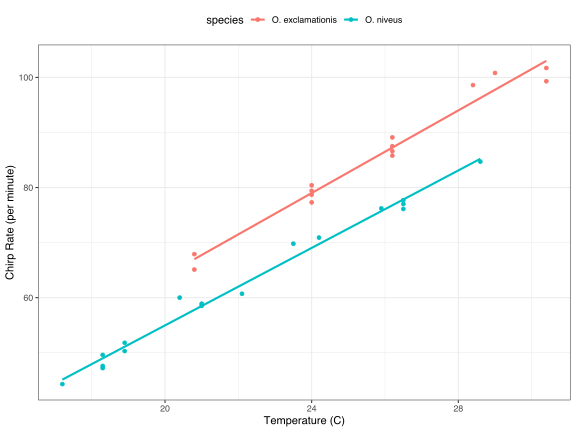
\includegraphics[width=1\linewidth]{figures/tidyverse-cricket-plot-1} \end{center}

The data show fairly linear trends for each species. For a given temperature, \emph{O. exclamationis} appears to have more chirps than the other species. For an inferential model, the researchers might have specified the following null hypotheses prior to seeing the data:

\begin{itemize}
\item
  Temperature has no affect on the chirp rate (denoted as hypothesis \#1)
\item
  There are no differences between the species in terms of chirp rate.
\end{itemize}

There may be some scientific rationale for being able to predict the chirp rate but the focus here will be on inference.

To fit an ordinary linear model, the \texttt{lm()} function is commonly used. The important arguments to this function are a model formula and a data frame that contains the data The formula is \emph{symbolic}. For example, the simple formula:

\begin{Shaded}
\begin{Highlighting}[]
\NormalTok{rate }\OperatorTok{~}\StringTok{ }\NormalTok{temp}
\end{Highlighting}
\end{Shaded}

states that the chirp rate is the outcome (since it is on the left-hand side of the tidle \texttt{\textasciitilde{}}) and that the temperature values are the predictor\footnote{Most model functions implicitly add an intercept column.}. Suppose the data contained the time of day in which the measurements were obtained in a column called \texttt{time}. The formula

\begin{Shaded}
\begin{Highlighting}[]
\NormalTok{rate }\OperatorTok{~}\StringTok{ }\NormalTok{temp }\OperatorTok{+}\StringTok{ }\NormalTok{time}
\end{Highlighting}
\end{Shaded}

would not add the time and temperature values together. This formula would symbolically represent that temperature and time should be added as a separate \emph{main effects} to the model. Main effects are model terms that contain a single predictor variable.

There are no time measurements in these data but the species can be added to the model in the same way:

\begin{Shaded}
\begin{Highlighting}[]
\NormalTok{rate }\OperatorTok{~}\StringTok{ }\NormalTok{temp }\OperatorTok{+}\StringTok{ }\NormalTok{species}
\end{Highlighting}
\end{Shaded}

Species is not a quantitative variable; in the data frame, it is represented as a factor column with levels \texttt{"O.\ exclamationis"} and \texttt{"O.\ niveus"}. The vast majority of model functions cannot operate on non-numeric data. For species, the model needs to \emph{encode} the species data into a numeric format. The most common approach is to use indicator variables (also known as ``dummy variables'') in place of the original qualitative values. In this instance, since species has two possible values, the model formula will automatically encode this column as numeric by adding a new column that has a value of zero when the species is \texttt{"O.\ exclamationis"} and a value of one when the data correspond to \texttt{"O.\ niveus"}. The underlying formula machinery will automatically convert these data for the data used to create the model as well as for any new data points (for example, when the model is used for prediction).

Suppose there were five species. The model formula would automatically add \emph{four} additional binary columns that are binary indicators for four of the species. The \emph{reference level} of the factor (i.e., the first level) is always left out of the predictor set. The idea is that, if you know the values of the four indicator variables, the value of the species can be determined.

The model formula shown above creates a model where there are different y-intercepts for each species. It is a reasonable supposition that the slopes of the regression lines could be different for each species. To accommodate this structure, an \emph{interaction} term can be added to the model. This can be specified in a few different ways, the most basic uses the colon:

\begin{Shaded}
\begin{Highlighting}[]
\NormalTok{rate }\OperatorTok{~}\StringTok{ }\NormalTok{temp }\OperatorTok{+}\StringTok{ }\NormalTok{species }\OperatorTok{+}\StringTok{ }\NormalTok{temp}\OperatorTok{:}\NormalTok{species}

\CommentTok{# A shortcut can be used to expand all interactions containing}
\CommentTok{# interactions with two variables:}
\NormalTok{rate }\OperatorTok{~}\StringTok{ }\NormalTok{(temp }\OperatorTok{+}\StringTok{ }\NormalTok{species)}\OperatorTok{^}\DecValTok{2}
\end{Highlighting}
\end{Shaded}

In addition to the convenience of automatically creating indicator variables, the formula offers a few other niceties:

\begin{itemize}
\item
  \emph{In-line} functions can be used in the formula. For example, if the natural log of the temperate were used, the formula \texttt{rate\ \textasciitilde{}\ log(temp)} could be used. Since the formula is symbolic by default, literal math can be done to the predictors using the identity function \texttt{I()}. For example, to use Fahrenheit units, the formula could be \texttt{rate\ \textasciitilde{}\ I(\ (temp\ *\ 9/5)\ +\ 32\ )} to make the conversion.
\item
  R has many functions that are useful inside of formulas. For example, \texttt{poly(x,\ 3)} would create linear, quadratic, and cubic terms for \texttt{x} to the model as main effects. Also, the \texttt{splines} package has several functions to create nonlinear spline terms in the formula.
\item
  For data sets where there are many predictors, the period shortcut is available. The period represents main effects for all of the columns that are not on the left-hand side of the tilde. For example, using \texttt{\textasciitilde{}\ (.)\^{}3} would create main effects as well as all two- and three-variable interactions to the model.
\end{itemize}

For the initial data analysis, the two-factor interaction model is used. In this book, the suffix \texttt{\_fit} is used for R objects for fitted models.

\begin{Shaded}
\begin{Highlighting}[]
\NormalTok{interaction_fit <-}\StringTok{  }\KeywordTok{lm}\NormalTok{(rate }\OperatorTok{~}\StringTok{ }\NormalTok{(temp }\OperatorTok{+}\StringTok{ }\NormalTok{species)}\OperatorTok{^}\DecValTok{2}\NormalTok{, }\DataTypeTok{data =}\NormalTok{ crickets) }

\CommentTok{# To print a short summary of the model:}
\NormalTok{interaction_fit}
\CommentTok{#> }
\CommentTok{#> Call:}
\CommentTok{#> lm(formula = rate ~ (temp + species)^2, data = crickets)}
\CommentTok{#> }
\CommentTok{#> Coefficients:}
\CommentTok{#>           (Intercept)                   temp  }
\CommentTok{#>               -11.041                  3.751  }
\CommentTok{#>      speciesO. niveus  temp:speciesO. niveus  }
\CommentTok{#>                -4.348                 -0.234}
\end{Highlighting}
\end{Shaded}

This output is a little hard to read. For the species indicator variables, R mashes the variable name (\texttt{species}) together with the factor level (\texttt{O.\ niveus}) with no delimiter.

Before going into any results for this model, the fit should be assessed using diagnostic plots. The \texttt{plot()} method for \texttt{lm} objects can be used. It produces a set of four plots for the object, each showing different aspects of the fit. Two plots are shown here:

\begin{Shaded}
\begin{Highlighting}[]
\CommentTok{# Place two plots next to one another:}
\KeywordTok{par}\NormalTok{(}\DataTypeTok{mfrow =} \KeywordTok{c}\NormalTok{(}\DecValTok{1}\NormalTok{, }\DecValTok{2}\NormalTok{))}

\CommentTok{# Show residuals vs predicted values:}
\KeywordTok{plot}\NormalTok{(interaction_fit, }\DataTypeTok{which =} \DecValTok{1}\NormalTok{)}

\CommentTok{# A normal quantile plot on the residuals:}
\KeywordTok{plot}\NormalTok{(interaction_fit, }\DataTypeTok{which =} \DecValTok{2}\NormalTok{)}
\end{Highlighting}
\end{Shaded}

\begin{center}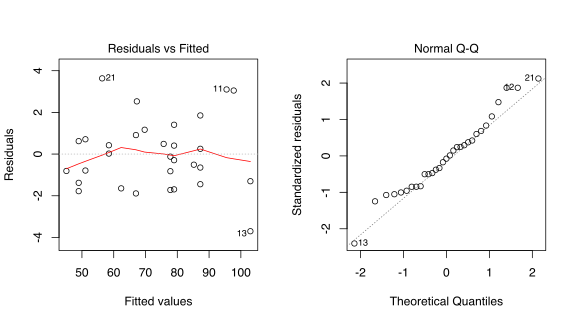
\includegraphics[width=1\linewidth]{figures/tidyverse-interaction-plots-1} \end{center}

These appear reasonable enough to conduct inferential analysis.

From a technical standpoint, R is \emph{lazy}. Model fitting functions typically compute the minimum possible quantities. For example, there may be interest in the coefficient table for each model term. This is not automatically computed but is instead computed via the \texttt{summary()} method.

Our second order of business is to assess if the inclusion of the interaction term is necessary. The most appropriate approach for this model is to re-compute the model without the interaction term and use the \texttt{anova()} method.

\begin{Shaded}
\begin{Highlighting}[]
\CommentTok{# Fit a reduced model:}
\NormalTok{main_effect_fit <-}\StringTok{  }\KeywordTok{lm}\NormalTok{(rate }\OperatorTok{~}\StringTok{ }\NormalTok{temp }\OperatorTok{+}\StringTok{ }\NormalTok{species, }\DataTypeTok{data =}\NormalTok{ crickets) }

\CommentTok{# Compare the two:}
\KeywordTok{anova}\NormalTok{(main_effect_fit, interaction_fit)}
\CommentTok{#> Analysis of Variance Table}
\CommentTok{#> }
\CommentTok{#> Model 1: rate ~ temp + species}
\CommentTok{#> Model 2: rate ~ (temp + species)^2}
\CommentTok{#>   Res.Df  RSS Df Sum of Sq    F Pr(>F)}
\CommentTok{#> 1     28 89.3                         }
\CommentTok{#> 2     27 85.1  1      4.28 1.36   0.25}
\end{Highlighting}
\end{Shaded}

The results of the statistical test generates a p-value of 0.3. This value implies that there is a lack of evidence for the alternative hypothesis that the the interaction term is needed by the model. For this reason, further analysis will be conducted on the model without the interaction.

Residual plots should be re-assessed to make sure that our theoretical assumptions are valid enough to trust the p-values produced by the model (not shown but spoiler alert: they are).

The \texttt{summary()} method is used to inspect the coefficients, standard errors, and p-values of each model term:

\begin{Shaded}
\begin{Highlighting}[]
\KeywordTok{summary}\NormalTok{(main_effect_fit)}
\CommentTok{#> }
\CommentTok{#> Call:}
\CommentTok{#> lm(formula = rate ~ temp + species, data = crickets)}
\CommentTok{#> }
\CommentTok{#> Residuals:}
\CommentTok{#>    Min     1Q Median     3Q    Max }
\CommentTok{#> -3.013 -1.130 -0.391  0.965  3.780 }
\CommentTok{#> }
\CommentTok{#> Coefficients:}
\CommentTok{#>                  Estimate Std. Error t value Pr(>|t|)}
\CommentTok{#> (Intercept)       -7.2109     2.5509   -2.83   0.0086}
\CommentTok{#> temp               3.6028     0.0973   37.03  < 2e-16}
\CommentTok{#> speciesO. niveus -10.0653     0.7353  -13.69  6.3e-14}
\CommentTok{#>                     }
\CommentTok{#> (Intercept)      ** }
\CommentTok{#> temp             ***}
\CommentTok{#> speciesO. niveus ***}
\CommentTok{#> ---}
\CommentTok{#> Signif. codes:  }
\CommentTok{#> 0 '***' 0.001 '**' 0.01 '*' 0.05 '.' 0.1 ' ' 1}
\CommentTok{#> }
\CommentTok{#> Residual standard error: 1.79 on 28 degrees of freedom}
\CommentTok{#> Multiple R-squared:  0.99,   Adjusted R-squared:  0.989 }
\CommentTok{#> F-statistic: 1.33e+03 on 2 and 28 DF,  p-value: <2e-16}
\end{Highlighting}
\end{Shaded}

From these values, the chirp rate for each species increases by 3.6 chirps as the temperature increases by a single degree. This term shows strong statistical significance as evidenced by the p-value. The species term has a value of -10.07. This indicates that, across all temperature values, \emph{O. niveus} is a chirp rate that is about 10 fewer chirps per minute. Similar to the temperature term, the species effect is associated with a very small p-value.

The only issue in this analysis is the intercept value. It indicates that at 0 C, there are -7.21 chirps per minute. While this is unreasonable, the data only go as low as 17.2 C and interpreting the model at 0 C would be an \emph{extrapolation}. This would be a bad idea. That said, the model fit is good within the \emph{applicable range} of the temperature values and the conclusions should be limited to the observed temperature range.

If there were a need to estimate the chirp rate at a temperature that was not observed in the experiment, the \texttt{predict()} method would be used. It takes the model object and a data frame of new values for prediction. For example, the model estimates the chirp rate for \emph{O. exclamationis} for temperatures between 15 C and 20 C can be computed via:

\begin{Shaded}
\begin{Highlighting}[]
\NormalTok{new_values <-}\StringTok{ }\KeywordTok{data.frame}\NormalTok{(}\DataTypeTok{species =} \StringTok{"O. exclamationis"}\NormalTok{, }\DataTypeTok{temp =} \DecValTok{15}\OperatorTok{:}\DecValTok{20}\NormalTok{)}
\KeywordTok{predict}\NormalTok{(main_effect_fit, new_values)}
\CommentTok{#>    1    2    3    4    5    6 }
\CommentTok{#> 46.8 50.4 54.0 57.6 61.2 64.8}
\end{Highlighting}
\end{Shaded}

Note that the non-numeric value of \texttt{species} is given to the predict method (as opposed to the binary indicator variable).

While this analysis has obviously not been an exhaustive demonstration of R's modeling capabilities, it does highlight some of the major features:

\begin{itemize}
\item
  The language has an expressive syntax for specifying model terms for simple and fairly complex models.
\item
  For formula method has many conveniences for modeling that are also applied to new data when predictions are generated.
\item
  There are numerous helper functions (e.g., \texttt{anova()}, \texttt{summary()} and \texttt{predict()}) that are used to conduct specific calculations after the fitted model is created.
\end{itemize}

Finally, as previously mentioned, this framework was devised in 1992. Most of the ideas and methods above were developed in that period and have remained remarkably relavant to this day. It highlights that the S language and, by extension R, has been designed as a language for data analysis since its inception.

\hypertarget{why-tidiness-is-important-for-modeling}{%
\section{Why tidiness is important for modeling}\label{why-tidiness-is-important-for-modeling}}

\hypertarget{some-additional-tidy-principals-for-modeling.}{%
\section{Some additional tidy principals for modeling.}\label{some-additional-tidy-principals-for-modeling.}}

\hypertarget{two-models}{%
\chapter{A tale of two models}\label{two-models}}

(tentative title)

Perhaps show an example of a predictive model and contrast it with another that is inferential.

Chicago data from FES: one predictive model and one to test if there is a difference in ridership with the Bears are at home. what do we care about for each? how accurate is the inferential model? Perhaps look at the \href{https://www.jstatsoft.org/article/view/v082i05}{\texttt{tscount}} package to deal with the autoregressive potential.

\hypertarget{data-spending}{%
\chapter{Spending our data}\label{data-spending}}

General data splitting

Re-emphasize roles or different data sets and good/bad ways of doing things.

Validation sets.

What we do differently with a lot of data.

Allude to resampling.

\hypertarget{model-metrics}{%
\chapter{How good is our model?}\label{model-metrics}}

(or how well does our model work? Superman does good; a model can work well)

Measuring performance

Don't revaluate the training set

Statistical significance as a measure of effectiveness.

\hypertarget{feature-engineering}{%
\chapter{Feature engineering}\label{feature-engineering}}

Purpose(s) of these activites.

Why do we do this?

Different representations of same data

Imputation; transformations; (unsup) removal; projection; encodings;

\hypertarget{workflows}{%
\chapter{A model workflow}\label{workflows}}

aka modeling process or model pipeline

How to encapsulate the pre-processing and model objects/activities

Treat them as a single unit for good methodology and convenience.

\hypertarget{resampling}{%
\chapter{Resampling for evaluating performance}\label{resampling}}

Maybe inlcude some simple examples of comparing models using resampling (perhaps go full \texttt{tidyposterior}?)

\bibliography{TMwR.bib}

\end{document}
